% Group 7 poster — DSC6007
% 编译：cd poster && latexmk -pdf poster.tex   （或 pdflatex poster.tex 两次）
\documentclass[10pt]{article}
\usepackage[a4paper,landscape,margin=0mm]{geometry}
\usepackage[T1]{fontenc}
\usepackage{newtxtext,newtxmath}          % Times New Roman 风格正文与数学
\usepackage[protrusion=true,expansion=true]{microtype}
\usepackage{xcolor}
\usepackage{booktabs,array,tabularx}
\usepackage{enumitem}
\usepackage{pgfplots}
\pgfplotsset{compat=1.18}
\usetikzlibrary{arrows.meta,positioning,calc,fit}
\usepackage[poster,skins,raster]{tcolorbox}
\pagestyle{empty}

% ---------------------------------------------------------------- 颜色
\definecolor{navy}{HTML}{1F3A5F}
\definecolor{accent}{HTML}{2F6690}
\definecolor{rnd}{HTML}{5B84B1}           % Random
\definecolor{bts}{HTML}{E0873A}           % Bernoulli TS
\definecolor{soft}{HTML}{EEF3F8}
\definecolor{note}{HTML}{555555}

% ---------------------------------------------------------------- 正文字号
\newcommand{\body}{\fontsize{8.2}{9.75}\selectfont}
\newcommand{\lead}[1]{\textbf{\color{navy}#1}\enspace}
\newcommand{\tnote}[1]{{\fontsize{7.2}{8.4}\selectfont\color{note}#1\par}}
\setlength{\parskip}{2.2pt}
\setlength{\parindent}{0pt}
\setlist{nosep,leftmargin=1.1em,label={\color{accent}\scriptsize$\blacktriangleright$}}
\renewcommand{\arraystretch}{1.12}
% 注意：tcbposter 的盒子里 tabular* 会报错，表格统一用 tabularx
\newcolumntype{R}{>{\raggedleft\arraybackslash}X}
\newcolumntype{C}{>{\centering\arraybackslash}X}
\setlength{\aboverulesep}{0.25ex}
\setlength{\belowrulesep}{0.35ex}

% 公式行距更紧凑
\AtBeginDocument{%
  \setlength{\abovedisplayskip}{2.5pt}\setlength{\belowdisplayskip}{2.5pt}%
  \setlength{\abovedisplayshortskip}{1pt}\setlength{\belowdisplayshortskip}{2.5pt}}

% 估计器卡片：名称 | 公式 | 说明
\newcommand{\est}[3]{%
  \begin{tcolorbox}[enhanced, colback=white, colframe=accent!35, boxrule=0.4pt, arc=1mm,
    borderline west={2pt}{0pt}{accent}, left=2mm, right=1.5mm, top=0.5mm, bottom=0.6mm,
    before skip=1.2mm, after skip=0mm, before upper=\body]
  \textbf{\color{navy}#1}\hfill$#2$\par\vspace{0.3mm}\tnote{#3}
  \end{tcolorbox}}

\newcommand{\pe}{\pi_e}
\newcommand{\pb}{\pi_b}

\begin{document}
\begin{tcbposter}[
  coverage={spread, interior style={fill=white}},
  poster={columns=3, rows=1, colspacing=4.5mm, rowspacing=3mm, showframe=false},
  boxes={enhanced, sharp corners,
    % 边框不能太细：低于 1 像素时部分 PDF 阅读器在缩放时会把它丢掉
    colback=white, colframe=navy!40, boxrule=0.8pt,
    colbacktitle=navy!7, coltitle=navy,
    % 浅色标题栏 + 左侧深蓝色条，减轻整页的深色块
    overlay={\fill[navy] (title.north west) rectangle ([xshift=1.4mm]title.south west);},
    fonttitle=\bfseries\fontsize{10.6}{12}\selectfont,
    titlerule=0pt, toptitle=1.3mm, bottomtitle=1.1mm, lefttitle=3mm,
    left=3mm, right=3mm, top=1.6mm, bottom=1.6mm,
    before upper=\body},
]

% ============================================================ 标题
\posterbox[blankest, interior engine=path, height=21mm, halign=center, valign=center,
  underlay={\fill[navy] (frame.south west) rectangle ([yshift=0.45mm]frame.south east);}]
  {name=title, column=1, span=3, below=top}{%
  {\fontsize{22}{26}\selectfont\bfseries\color{navy} Offline Policy Evaluation with Real-World Bandit Logs\par}
  \vspace{2.2mm}
  {\fontsize{10.5}{12}\selectfont Jingzhe FENG \quad Jun LI \quad Kaiwen WANG \quad Siyu YAN \quad Zenghuan WANG\par}
  \vspace{1mm}
  {\fontsize{9}{11}\selectfont\color{note} Group 7 \quad$\cdot$\quad DSC6007: Dynamic Programming and Reinforcement Learning\par}
}

% ============================================================ 页脚
\posterbox[blankest, height=7mm, valign=center, left=0mm, right=0mm, before upper={}]
  {name=refs, column=1, span=3, above=bottom}{%
  {\fontsize{6.6}{8}\selectfont\color{note}
  \textbf{References.} Saito et al.\ (2020), \emph{A Large-scale Open Dataset for Bandit Algorithms};
  Saito et al.\ (2021), \emph{Open Bandit Pipeline};
  Dudík et al.\ (2011), doubly robust policy evaluation;
  Swaminathan \& Joachims (2015), self-normalized importance sampling.\par}
}

% ============================================================ 1 背景
\posterbox[adjusted title={1\quad Background and research objective}]
  {name=bg, column=1, below=title}{%
\lead{Motivation.}Contextual bandits select items to maximize immediate click reward.
Online tests expose users to unproven policies; \emph{off-policy evaluation} (OPE)
estimates a new policy's value from historical interactions before deployment.

\lead{Problem.}Only the displayed item's reward is observed. A new policy changes action
probabilities, so the logged average reward does not directly estimate its value.
Small logging probabilities can give a few observations excessive influence.

\lead{Objective.}Compare DM, IPS, SNIPS and DR under policy mismatch, and study how sample
size and weight clipping affect estimation error, stability and candidate-policy rankings.

\begin{tcolorbox}[enhanced, colback=soft, colframe=soft, arc=1mm, boxrule=0pt,
  left=1mm, right=1mm, top=0.5mm, bottom=0.5mm, before upper=\body]
\centering Target value:\quad
$V(\pe) = \mathbb{E}_{x}\Bigl[\,\sum_{a} \pe(a\mid x)\,\mathbb{E}[r\mid x,a]\Bigr]$
\end{tcolorbox}
}

% ============================================================ 2 数据
\posterbox[adjusted title={2\quad Dataset and preprocessing}]
  {name=data, column=1, between=bg and refs}{%
\textbf{26.9 million} ZOZOTOWN recommendation records (24--30 Nov 2019), with
\textcolor{rnd}{\textbf{Uniform Random}} and \textcolor{bts}{\textbf{Bernoulli Thompson Sampling (BTS)}}
logs for three campaigns and three display positions.

\begin{center}
\begin{tabularx}{\linewidth}{@{}lRRR@{}}
\toprule
\textbf{Campaign} & \textbf{Items} & \textbf{Random test} & \textbf{BTS test}\\
\midrule
All   & 80 & 412{,}250 & 3{,}706{,}504\\
Men   & 34 & 135{,}860 & 1{,}223{,}053\\
Women & 46 & 259{,}334 & 2{,}329{,}202\\
\bottomrule
\end{tabularx}
\end{center}
\vspace{-1mm}

\lead{Recorded variables.}User context $x$, displayed item $a$, position, binary click $r$
and logging propensity $\pb(a\mid x)$; position is part of the conditioning context.
Clicks are rare in the test sets, so uncertainty estimates matter.

\lead{Cleaning.}Validate actions, clicks and probabilities; remove exact duplicates
(${\approx}\,0.02\%$); align item-category encodings between the two logging policies.

\lead{Features and split.}
\begin{itemize}
\item Chronological split: first 70\% of each log for training, last 30\% for testing.
\item Encoders fitted on Random train only; categories one-hot, affinities $\log(1{+}\cdot)$ and normalized.
\item Context dimensions: 116 / 69 / 80 (All / Men / Women).
\item Propensities preserved unclipped for the clipping experiments.
\end{itemize}
}

% ============================================================ 3 估计器
\posterbox[adjusted title={3\quad Off-policy estimators}]
  {name=est, column=2, below=title}{%
Let $\pe(a\mid x)$ be the target policy and $\pb(a\mid x)$ the logging policy. Define the
importance weight $w_i$, reward prediction $q_i$ and target-averaged prediction $m_i$:
\[
w_i=\frac{\pe(a_i\mid x_i)}{\pb(a_i\mid x_i)},\quad
q_i=\hat q(x_i,a_i),\quad
m_i=\textstyle\sum_{a}\pe(a\mid x_i)\,\hat q(x_i,a).
\]
\tnote{\centering Overlap requires $\pb(a\mid x)>0$ wherever $\pe(a\mid x)>0$.}

\est{DM\,: direct method}{\hat V_{\mathrm{DM}}=\tfrac1n\textstyle\sum_i m_i}
  {Uses predicted rewards for every action. Low variance, but model misspecification can bias the estimate.}
\est{IPS\,: inverse propensity scoring}{\hat V_{\mathrm{IPS}}=\tfrac1n\textstyle\sum_i w_i r_i}
  {Unbiased with correct propensities and action overlap. Extreme weights can create high variance.}
\est{SNIPS\,: self-normalized IPS}{\hat V_{\mathrm{SNIPS}}=\textstyle\sum_i w_i r_i\big/\sum_i w_i}
  {Normalizes total weight and often improves stability, at the cost of finite-sample bias.}
\est{DR\,: doubly robust}{\hat V_{\mathrm{DR}}=\tfrac1n\textstyle\sum_i\bigl[m_i+w_i(r_i-q_i)\bigr]}
  {Predictions plus weighted residuals. A correct reward model \emph{or} correct propensities suffice, given overlap.}
}

% ============================================================ 4 实验设计
\posterbox[adjusted title={4\quad Experimental design \textmd{\small(planned)}}]
  {name=design, column=2, between=est and refs}{%
\lead{Candidate policies.}Train \textbf{LinUCB} (uncertainty bonus on predicted reward) and
\textbf{LogisticTS} (posterior sampling of click-model parameters) on Random train, then
freeze them so test data stay separate from learning.

\begin{center}
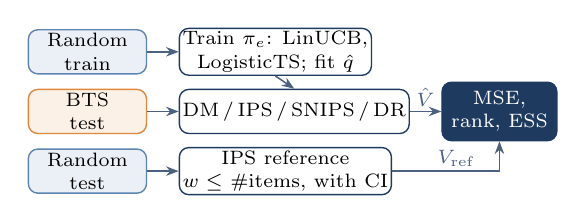
\begin{tikzpicture}[
  font=\fontsize{7.2}{8.4}\selectfont,
  data/.style={draw=#1, fill=#1!12, rounded corners=1.2mm, minimum width=15mm, minimum height=5.6mm, align=center, line width=0.5pt, inner sep=1.2pt},
  proc/.style={draw=navy, fill=white, rounded corners=1.2mm, minimum width=24mm, minimum height=5.6mm, align=center, line width=0.5pt, inner sep=1.2pt},
  outp/.style={draw=navy, fill=navy, text=white, rounded corners=1.2mm, minimum width=14mm, minimum height=5.6mm, align=center},
  arr/.style={-{Stealth[length=1.6mm]}, line width=0.55pt, color=navy!80},
  node distance=1.8mm and 4mm]
  \node[data=rnd]                 (rtr) {Random\\train};
  \node[proc, right=of rtr]       (pol) {Train $\pe$: LinUCB,\\LogisticTS; fit $\hat q$};
  \node[data=bts, below=of rtr]   (bte) {BTS\\test};
  \node[proc, right=of bte]       (ope) {DM\,/\,IPS\,/\,SNIPS\,/\,DR};
  \node[data=rnd, below=of bte]   (rte) {Random\\test};
  \node[proc, right=of rte]       (ref) {IPS reference\\$w\le$ \#items, with CI};
  \node[outp, right=of ope]       (cmp) {MSE,\\rank, ESS};
  \draw[arr] (rtr) -- (pol);
  \draw[arr] (bte) -- (ope);
  \draw[arr] (rte) -- (ref);
  \draw[arr] (pol.south) -- (ope.north);
  \draw[arr] (ope) -- node[above,inner sep=1.5pt]{$\hat V$} (cmp);
  \draw[arr] (ref.east) -| node[pos=0.3,above,inner sep=1.5pt]{$V_{\mathrm{ref}}$} (cmp.south);
\end{tikzpicture}
\end{center}
\vspace{-1.5mm}

\lead{Reference.}For each new policy, IPS on independent Random test logs: uniform logging
bounds weights by the number of items. The reference has sampling error, so it carries an
uncertainty interval.

\lead{Sensitivity analysis.}Vary sample size and clipping threshold $c$ via $\min(w_i,c)$;
repeat subsampling to measure the bias--variance trade-off, monitoring
$\mathrm{ESS}=(\sum_i w_i)^2/\sum_i w_i^2$.
\textit{Sanity check:} a uniform target policy should reproduce Random CTR.
}

% ============================================================ 5 初步结果
\posterbox[adjusted title={5\quad Preliminary results \textmd{\small(completed)}}]
  {name=res, column=3, below=title}{%
Observed test CTR (\%) with 95\% Wilson intervals; each policy is evaluated on its own test logs.

\begin{center}
\begin{tabularx}{\linewidth}{@{}lCCr@{}}
\toprule
\textbf{Campaign} & \textcolor{rnd}{\textbf{Random}} & \textcolor{bts}{\textbf{BTS}} & \textbf{Lift}\\
\midrule
All   & 0.347 {\color{note}\scriptsize[0.330, 0.366]} & 0.491 {\color{note}\scriptsize[0.484, 0.498]} & +41.4\%\\
Men   & 0.541 {\color{note}\scriptsize[0.503, 0.581]} & 0.665 {\color{note}\scriptsize[0.650, 0.679]} & +22.9\%\\
Women & 0.487 {\color{note}\scriptsize[0.461, 0.515]} & 0.637 {\color{note}\scriptsize[0.627, 0.648]} & +30.7\%\\
\bottomrule
\end{tabularx}
\end{center}
\vspace{-2mm}

\begin{center}
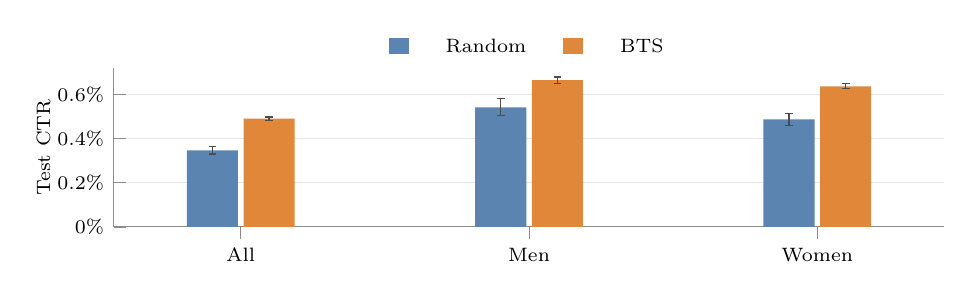
\begin{tikzpicture}
\begin{axis}[
  width=\linewidth, height=36mm,
  ybar, bar width=6.5mm, enlarge x limits=0.22,
  ymin=0, ymax=0.72, ytick={0,0.2,0.4,0.6},
  yticklabel={\pgfmathprintnumber[fixed,precision=1]{\tick}\%},
  symbolic x coords={All,Men,Women}, xtick=data,
  tick label style={font=\fontsize{7.4}{8}\selectfont},
  ylabel={Test CTR}, ylabel style={font=\fontsize{7.4}{8}\selectfont, yshift=-1.5mm},
  axis line style={draw=black!45}, tick style={draw=black!45},
  ymajorgrids, grid style={draw=black!10},
  axis x line*=bottom, axis y line*=left,
  legend style={font=\fontsize{7.4}{8}\selectfont, draw=none, fill=none,
    at={(0.5,1.0)}, anchor=south, legend columns=2, column sep=4mm},
  legend image code/.code={\fill[#1] (0cm,-0.08cm) rectangle (0.25cm,0.12cm);},
  error bars/y dir=both, error bars/y explicit,
  error bars/error bar style={line width=0.6pt, black!70},
  error bars/error mark options={rotate=90, mark size=1.4pt, black!70},
]
\addplot[fill=rnd, draw=none] coordinates {
  (All,0.347)   += (0,0.019) -= (0,0.017)
  (Men,0.541)   += (0,0.040) -= (0,0.038)
  (Women,0.487) += (0,0.028) -= (0,0.026)};
\addplot[fill=bts, draw=none] coordinates {
  (All,0.491)   += (0,0.007) -= (0,0.007)
  (Men,0.665)   += (0,0.014) -= (0,0.015)
  (Women,0.637) += (0,0.011) -= (0,0.010)};
\legend{Random, BTS}
\end{axis}
\end{tikzpicture}
\end{center}
\vspace{-2mm}

BTS achieves a relatively \textbf{41.4\%}, \textbf{22.9\%} and \textbf{30.7\%} higher CTR in All,
Men and Women. These on-policy benchmarks do not yet determine the most accurate OPE estimator.
}

% ============================================================ 6 评估与结论
\posterbox[adjusted title={6\quad Evaluation plan and conclusion}]
  {name=eval, column=3, between=res and refs}{%
Compare DM, IPS, SNIPS and DR across campaigns and policy settings, using repeated
subsamples to report error and uncertainty.

\begin{center}
\begin{tabularx}{\linewidth}{@{}>{\bfseries}lX@{}}
\toprule
Metric & \textbf{What it measures}\\
\midrule
MSE             & Mean squared error vs.\ reference\\
Bias / variance & Systematic error / sampling variability\\
Spearman rank   & Agreement in policy ranking\\
ESS             & Effective sample size under unequal weights\\
\bottomrule
\end{tabularx}
\end{center}
\vspace{-1mm}

\begin{tcolorbox}[enhanced, colback=soft, colframe=soft, arc=1mm, boxrule=0pt,
  borderline west={2pt}{0pt}{navy}, left=2mm, right=1.5mm, top=1mm, bottom=1mm,
  before upper=\body]
\lead{Conclusion so far.}BTS beats Random on CTR in all campaigns, but on-policy CTR cannot rank OPE estimators.
\lead{Strengths.}Real industrial logs, an independent Random reference, uncertainty throughout.
\lead{Limits.}Sparse clicks, weak overlap, propensities down to $10^{-6}$.
\lead{Outlook.}Finish the MSE, ranking and clipping study; extend to Switch-DR.
\end{tcolorbox}
}

\end{tcbposter}
\end{document}
